% !TeX program = pdfLaTeX
\documentclass[smallextended]{svjour3}       % onecolumn (second format)
%\documentclass[twocolumn]{svjour3}          % twocolumn
%
\smartqed  % flush right qed marks, e.g. at end of proof
%
\usepackage{amsmath}
\usepackage{graphicx}
\usepackage[utf8]{inputenc}

\usepackage[hyphens]{url} % not crucial - just used below for the URL
\usepackage{hyperref}
\providecommand{\tightlist}{%
  \setlength{\itemsep}{0pt}\setlength{\parskip}{0pt}}

%
% \usepackage{mathptmx}      % use Times fonts if available on your TeX system
%
% insert here the call for the packages your document requires
%\usepackage{latexsym}
% etc.
%
% please place your own definitions here and don't use \def but
% \newcommand{}{}
%
% Insert the name of "your journal" with
% \journalname{myjournal}
%

%% load any required packages here




\usepackage{kotex}
\usepackage{cite}
\usepackage{booktabs}
\usepackage{longtable}
\usepackage{array}
\usepackage{multirow}
\usepackage{wrapfig}
\usepackage{float}
\usepackage{colortbl}
\usepackage{pdflscape}
\usepackage{tabu}
\usepackage{threeparttable}
\usepackage{threeparttablex}
\usepackage[normalem]{ulem}
\usepackage{makecell}
\usepackage{xcolor}

\begin{document}

\title{사람과 기계의 일자리 경쟁 요인과 협업 방안 }



\author{  이광춘 \and  주용우 \and  }


\institute{
        이광춘 \at
     연세대학교 상경대학 응용통계학과 \\
     \email{\href{mailto:kwangchun.lee.7@gmail.com}{\nolinkurl{kwangchun.lee.7@gmail.com}}}  %  \\
%             \emph{Present address:} of F. Author  %  if needed
    \and
        주용우 \at
     연세대학교 상경대학 응용통계학과 \\
     \email{\href{mailto:yongwoo96@yonsei.ac.kr}{\nolinkurl{yongwoo96@yonsei.ac.kr}}}  %  \\
%             \emph{Present address:} of F. Author  %  if needed
    \and
    }

\date{Received: date / Accepted: date}
% The correct dates will be entered by the editor


\maketitle

\begin{abstract}
기계는 단순히 사칙 연산, 문서 작업으로 사용되어 왔다. 그러나 기술 발전을
시작으로 인공지능 세대가 열리며 기계는 단순히 계산만 할 수 있는 도구가
아니라 사람의 언어를 이해하고 소통할 수 있는 자연어 처리 기술 또는
사람의 의존도가 높았던 영상 분야 등 다양한 분야에 상용화되기 시작했다.
2016년 인공지능 바둑 프로그램 `알파고'가 이세돌 9단을 현격한 기량 차이로
격파하면서 인공지능에 대한 관심이 급격히 증가하였다. 기계는 우수한
성능을 저렴한 가격에 사용할 수 있으며 경쟁력을 보여 인간의 일자리를
대체하기 시작했다. 그러나 인공지능은 오랜 학습을 토대로 기능을 향상
시키므로 전문성 측면에서는 인간이 더 우수하다. 인공지능을 사용함으로서
인간의 일자리에 주는 영향과 앞으로 어떤 방식으로 기계와 인간이 협력해
효율적으로 생산성을 높일 수 있는지에 대한 방안을 제시하고자 한다.
\\
\keywords{
        자동화 \and
        데이터 과학 \and
        인공지능 \and
        일자리 \and
        기계와 사람의 업무분장 \and
    }


\end{abstract}


\def\spacingset#1{\renewcommand{\baselinestretch}%
{#1}\small\normalsize} \spacingset{1}


\hypertarget{intro}{%
\section{들어가며}\label{intro}}

과거에는 숫자를 다룰 수 있는 사람만이 암산으로 숫자 계산을 할 수 있었다.
그러나 주판의 탄생으로 주판을 사용하는 사람과 사용하지 못하는 사람의
생산성은 차이를 들어내기 시작했으며 18세기 사이 1차 산업혁명의 시작으로
생산성의 중요성은 더욱 높아졌다. 그리고 영국 수학자인 찰스 배비지가
기계장치 계산기의 발명으로 기계를 사용하여 사칙연산을 사람들보다 빨리
처리해 생산성과 정확도를 높이는 방법을 연구하기 시작했다.

\begin{center}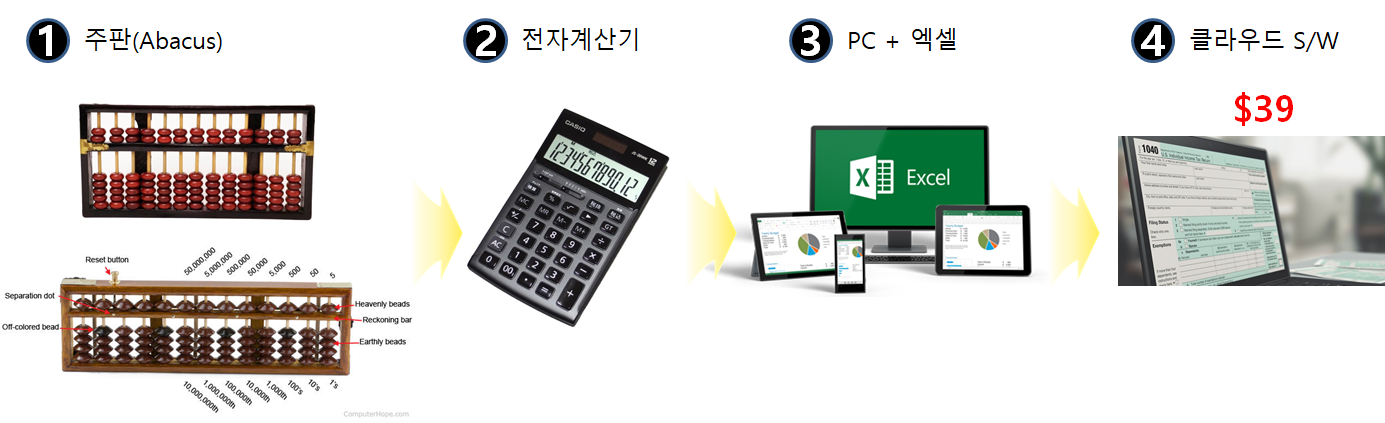
\includegraphics[width=1\linewidth]{fig/tax-preparation} \end{center}

그 이후 개인용 컴퓨터 사용이 확산되고 바지칼크와 로터스 1-2-3의 개발로
표 형식으로 데이터를 저장하고 계산할 수 있는 스프레드시트를 사용하기
시작했다. 그리고 마이크로소프트에서 개발한 엑셀 스프레드시트 프로그램은
대부분 모든 분야에 상용화가 되었으며 데이터 정리, 계산, 분석 등 생산성과
효율성 상향에 긍정적인 영향을 미쳤다. 예를 들면 숫자 계산 업무가 많은
세무사들은 엑셀 프로그램을 통해 계산 처리 시간을 단축하면서 생산성을
높여왔다. 그러나 세무사가 해오던 업무를 PC매거진 \cite{yakal_2020}에
소개된 세금관련 프로그램이 이제는 \$39 (약 4만원)에 사용할 수 있게
되었다. 1년치 세무 업무를 약 4만원을 지불해 계속 사용하게 되면 세무사의
의존도는 낮아진다. 핵심은 자동화된 기계와의 경쟁에서 사람이 승리할 수
있을지가 의문이다.

CPU (Central Processing Unit, 중앙 처리 장치), GPU (Graphics Processing
Unit, 그래픽 처리 장치), 메모리, 다중 처리 등 기술의 발전으로 기계는
초당 몇 천 건의 업무를 처리할 수 있게 되었다. 그 결과 수학적 계산이 많이
필요한 인공지능의 활용이 시작하게 되었다. 인공지능 (AI, Artificial
Intelligence)은 기계가 경험을 통해 학습하고 기존에 보유한 지식을
조정하며 사람과 같은 방식으로 업무를 수행할 수 있도록 보조하는 기술이다
{[}SAS 인사이트{]}. 인공지능의 기술이 발전되면서 전에는 기계를 사용해서
숫자 연산 또는 문서 작업들 한계가 있었지만 이제는 사람들이 보는 글을
자연어 처리 (NLP, Natural Language Processing) 기술을 통해 사람처럼
이해하고 질문들을 물어보며 사람과 대화 하듯이 답을 알려준다. 그 외에도
전에는 접근하기 힘든 이미지 인식 기술도 인공지능을 통해 사람이 보지 못한
부분을 찾아주고 분석해 주거나 영상 보정을 하기 위해 많은 인력이 필요했던
부분도 이제는 인공지능 기술을 사용해 간편하고 신속히 해결할 수 있게
되었다. 그 결과, 숫자를 많이 다루는 세무사, 회계사 또는 문서 작업을
다루는 법률/변호사 일자리 외에도 시각 인지 업무가 중요한 의사 직종 등
다양한 측면의 직업들을 위협하기 시작했다. 가속도가 붙은 인공지능의
상용화의 이유 그리고 과연 이 기술이 모든 일자리를 대처할 수 있는지
알아보려고 한다.

\hypertarget{challenge-to-human}{%
\section{인공지능에 대체되는 일자리}\label{challenge-to-human}}

기계\cite{brynjolfsson2014second, ford2015rise, kaplan2015humans, chang_2017}는
빠르게 부상하고 있으며 비교적으로 직업 능력이 낮은 기계 조립 같은
분야에는 인공지능 기술이 일자리를 대체하기 시작했다. 그러나 바둑 역사상
최고의 기사 이창호를 이기고 최강자에 굴림해온 전설적인 이세돌 9 단이
구글 (Google)의 자회사 딥마인가 개발한 인공지능 바둑 프로그램 `알파고'에
패배하며 인공지능의 한계가 어디까지인지 의문을 남기며 전세계를 충격에
빠뜨렸다.

\begin{center}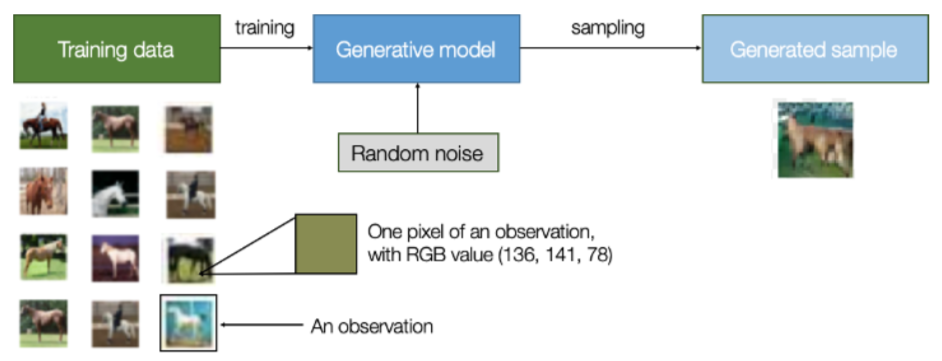
\includegraphics[width=0.49\linewidth]{fig/generative-model} \end{center}

\begin{center}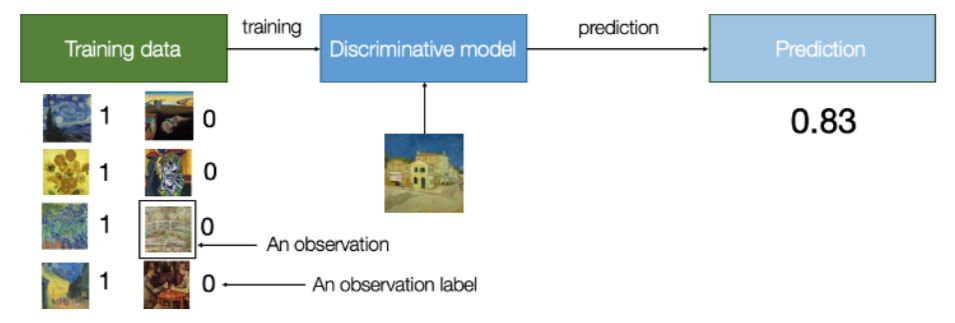
\includegraphics[width=0.49\linewidth]{fig/discriminative-model} \end{center}

대부분의 사람은 오감(시각, 후각, 청각, 촉각, 미각) 중에서 시각을 가장
중요한 감각이라고 꼽는다. 그 이유는 감각기관을 통해서 획득하는 정보의
90\% 이상이 시각을 통해서 얻어진다. 그래서 인간이 기계에 비해 유일하게
절대우위였던 부분은 시각 지능이었다. 그러므로 창작은 기계가 범접할 수
없는 고유한 인간의 영역이라고 믿어졌지만, 생성적 적대 신경망
\textbf{GAN(Generative Adversarial Network)}
\cite{brownlee_2019, hui_2018}의 등장으로 창작, 예술 분야에도 인간의
응전이 요구되기 시작했다. GAN은 이안 굿펠로우(Ian Goodfellow)가 신경
정보처리 시스템 학회 (NeurIPS) 에서 발표한 뒤로 딥러닝의 대가인 얀
르쿤(Yann Lecun) 교수도 GAN을 최근 10년간 머신러닝 연구 중 가장 혁신적인
아이디어로 극찬했다.

그림을 그리는 것은 `화가'라는 전업 직업을 만들 만큼 인간 고유의 영역으로
생각되었으나 인공지능 기술을 통해 아래와 같이 인간의 시각 지능 영역에도
영향을 주기 시작했다.

\begin{itemize}
\item
  이미지 생성(Image generation): GAN을 사용하여 기계가 이미지를 자동으로
  생성할 수 있다. 예를 들어 자동 로고생성기 등.
  \href{https://github.com/alex-sage/logo-gen}{GitHub:
  alex-sage/logo-gen}
\item
  텍스트로 이미지 합성 (Text-to-image synthesis): 영화 산업에서
  시나리오가 있는 상태에서 텍스트를 기초로 하여 이미지를 자동 생성시킴.
  \href{https://medium.com/datadriveninvestor/text-to-image-synthesis-6e5de1bf86ec}{Nikunj
  Gupta, ``Text-to-Image Synthesis'', Medium},
  \href{https://github.com/crisbodnar/text-to-image}{GitHub,
  text-to-image}
\item
  얼굴 노화(Face Aging): 연애 산업과 보안 산업에서 특히 유용한데 보안의
  경우 얼굴 노화과정을 GAN을 통해 모델을 갖춤으로써 직원의 노화에 따라
  신규 시스템으로 바꿀 필요가 없다.
  \href{https://github.com/yuanzhaoYZ/Face-Aging-CAAE}{GitHub,
  yuanzhaoYZ/Face-Aging-CAAE}
\item
  이미지를 다른 이미지로 번역(image-to-image-translation): 흑백이미지를
  칼러 이미지로, 스케치 이미지를 색칠된 이미지로, 이미지를 피카소나
  반고흐 스타일로 번역하는 것을 통해 시간을 상당히 줄일 수 있다.
  \href{https://github.com/topics/image-to-image-translation}{GitHub
  topics: image-to-image-translation}
\item
  고화질 이미지 생성(High-resolution image generation): 저해상도 카메라
  이미지를 고화질 이미지로 변환.
  \href{https://github.com/david-gpu/srez}{david-gpu/srez}
\item
  결측된 이미지 채워넣기(completing missing parts of images),
  \href{https://github.com/topics/image-completion}{Github topic:
  image-completion}: 이미지의 빠진 부분을 채워넣거나 불필요한 부분이
  있다면 지워서 결측시킨 후에 이미지를 채워넣는다.
\end{itemize}

인공지능은 이미지 분야 외에도 자연스럽게 사람들이 사용하는 자연어에도
적용하기 시작했다. 인공지능을 활용한 저작은 소프트웨어 개발자들이 소스
코드를 공유하는 인터넷 사이트 GitHub에도 특별한 주제로 다룰 만큼 다양한
프로젝트가 진행되고 있다. 그리고 기계는 텍스트 생성 외에도 음악을 만드는
것도 가능해졌다. 인공지능을 활용하는 추세가 대세를 잡으면서 빅데이터를
축적하고 클라우드 기반 기술을 활용하여 인공지능 모형을 만들 수 있는
토대가 마련되기 시작했다. 그 결과 기계로 텍스트 외에도 그림도 생성하고
음악도 제작이 가능해지면서 이를 조합해 연극 또는 영화 제작도 가능한
시대가 열리면서 인간의 직업을 위협하기 시작했다.

\begin{itemize}
\tightlist
\item
  \href{https://github.com/topics/text-generation}{GitHub topic:
  text-generation}

  \begin{itemize}
  \tightlist
  \item
    \href{https://github.com/Maluuba/newsqa}{Maluuba NewsQA dataset}
  \item
    \href{https://github.com/Maluuba/qgen-workshop}{Multi-task Question
    and Answer Generation}
  \end{itemize}
\item
  음악(music)

  \begin{itemize}
  \tightlist
  \item
    \href{https://salu133445.github.io/musegan/}{museGAN}
  \item
    \href{https://medium.com/@rachelchen_49210/generating-ambient-noise-from-wavenet-95aa7f0a8f77}{Rachel
    Chen (Dec 13, 2017), ``Generating Ambient Music from WaveNet'',
    Medium}
  \item
    \href{https://github.com/tensorflow/magenta}{tensorflow/magenta}
  \item
    \href{https://towardsdatascience.com/generating-pokemon-inspired-music-from-neural-networks-bc240014132}{Abraham
    Khan(Dec 15, 2018), ``Generating Pokemon-Inspired Music from Neural
    Networks'', Medium}
  \end{itemize}
\item
  연극(play)

  \begin{itemize}
  \tightlist
  \item
    \href{https://worldmodels.github.io/}{World Models}
  \item
    \href{https://dylandjian.github.io/world-models/}{Dylan's blog (June
    06, 2018), ``World Models applied to Sonic''}
  \end{itemize}
\end{itemize}

\hypertarget{automation-job-statistics}{%
\section{일자리 변동 원인}\label{automation-job-statistics}}

기계(Machine)라 하면 기계장치를 떠올릴 수 있지만, 영어로 머신(machine)
은 인공지능을 탑재한 컴퓨터로도 의미한다. 자동화 수준을 기계의 도움없이
모든 결정과 행동을 사람이 취하는 수준과, 인간을 배제하고 기계가 모든
의사결정을 내리고 자율적으로 운전, 판결, 세금계산 등 완전한 자동화
수준으로 나눌 수 있다\cite{cummings2014man}. 이미 사회에 많은 부분이
인공지능을 통한 자동화가 되었거나 아니면 자동화가 진행 중이거나 혹은
완전한 자동화가 진행되었다. 그 외에도 과거에는 세계화 전략을 통한 제조와
생산에 필요한 인력을 인건비가 저렴한 해외에서 찾았으나 인공지능 기술의
진화로 생산과 제조, 유통은 물론 마케팅과 고객 서비스 등 다양한 분야에서
경쟁적이고 효율적으로 사용이 가능해져 일자리에 커다란 변화가 생기기
시작했다.

\begin{table}[H]
\centering
\resizebox{\linewidth}{!}{
\begin{tabular}{rl}
\toprule
자동화 수준 & 자동화 수준 설명\\
\midrule
\rowcolor{gray!6}  1 & 컴퓨터는 어떤 도움도 주고 있지 못함: 사람이 모든 결정을 해야하고 행동도 취해야 함\\
2 & 컴퓨터가 대안이 될 수 있는 의사결정 목록과 행동목록을 제시함\\
\rowcolor{gray!6}  3 & 선택지를 몇개로 줄여줌\\
4 & 대안을 제시함\\
\rowcolor{gray!6}  5 & 사람이 승인하면 제안된 것을 실행함.\\
\addlinespace
6 & 자동 실행하기 전에 사람에게 거부권을 행사할 시간을 부여함\\
\rowcolor{gray!6}  7 & 자동으로 실행하고 나서, 필요할 때만 인간에게 통보함\\
8 & 컴퓨터가 요청을 받을 때만 인간에게 통보함\\
\rowcolor{gray!6}  9 & 컴퓨터가 결정을 내려야 될 때만, 인간에게 통보함\\
10 & 인간을 배제하고, 컴퓨터가 모든 결정을 내리고 행동도 자율적으로 취함.\\
\bottomrule
\end{tabular}}
\end{table}

\hypertarget{strategy-change}{%
\subsection{소싱전략의 변화}\label{strategy-change}}

Kinetics consulting services / Automation Anywhere 자료에 의하면 사무
로봇을 사용하면 비정규직 인력 아웃소싱 비용을 현재 시점보다 더욱 줄일 수
있다는 조사결과를 제시하고 있다. 예를 들면 미국, 영국, 호주 등 업무지원
인력 비용이 높은 선진국들은 경쟁력을 갖추고자 인력비용이 상대적으로 낮은
필리핀, 인도 등 영어가 가능하고 24시간 고객지원이 가능한 나라로 소싱
전략을 변경했었다.

\begin{center}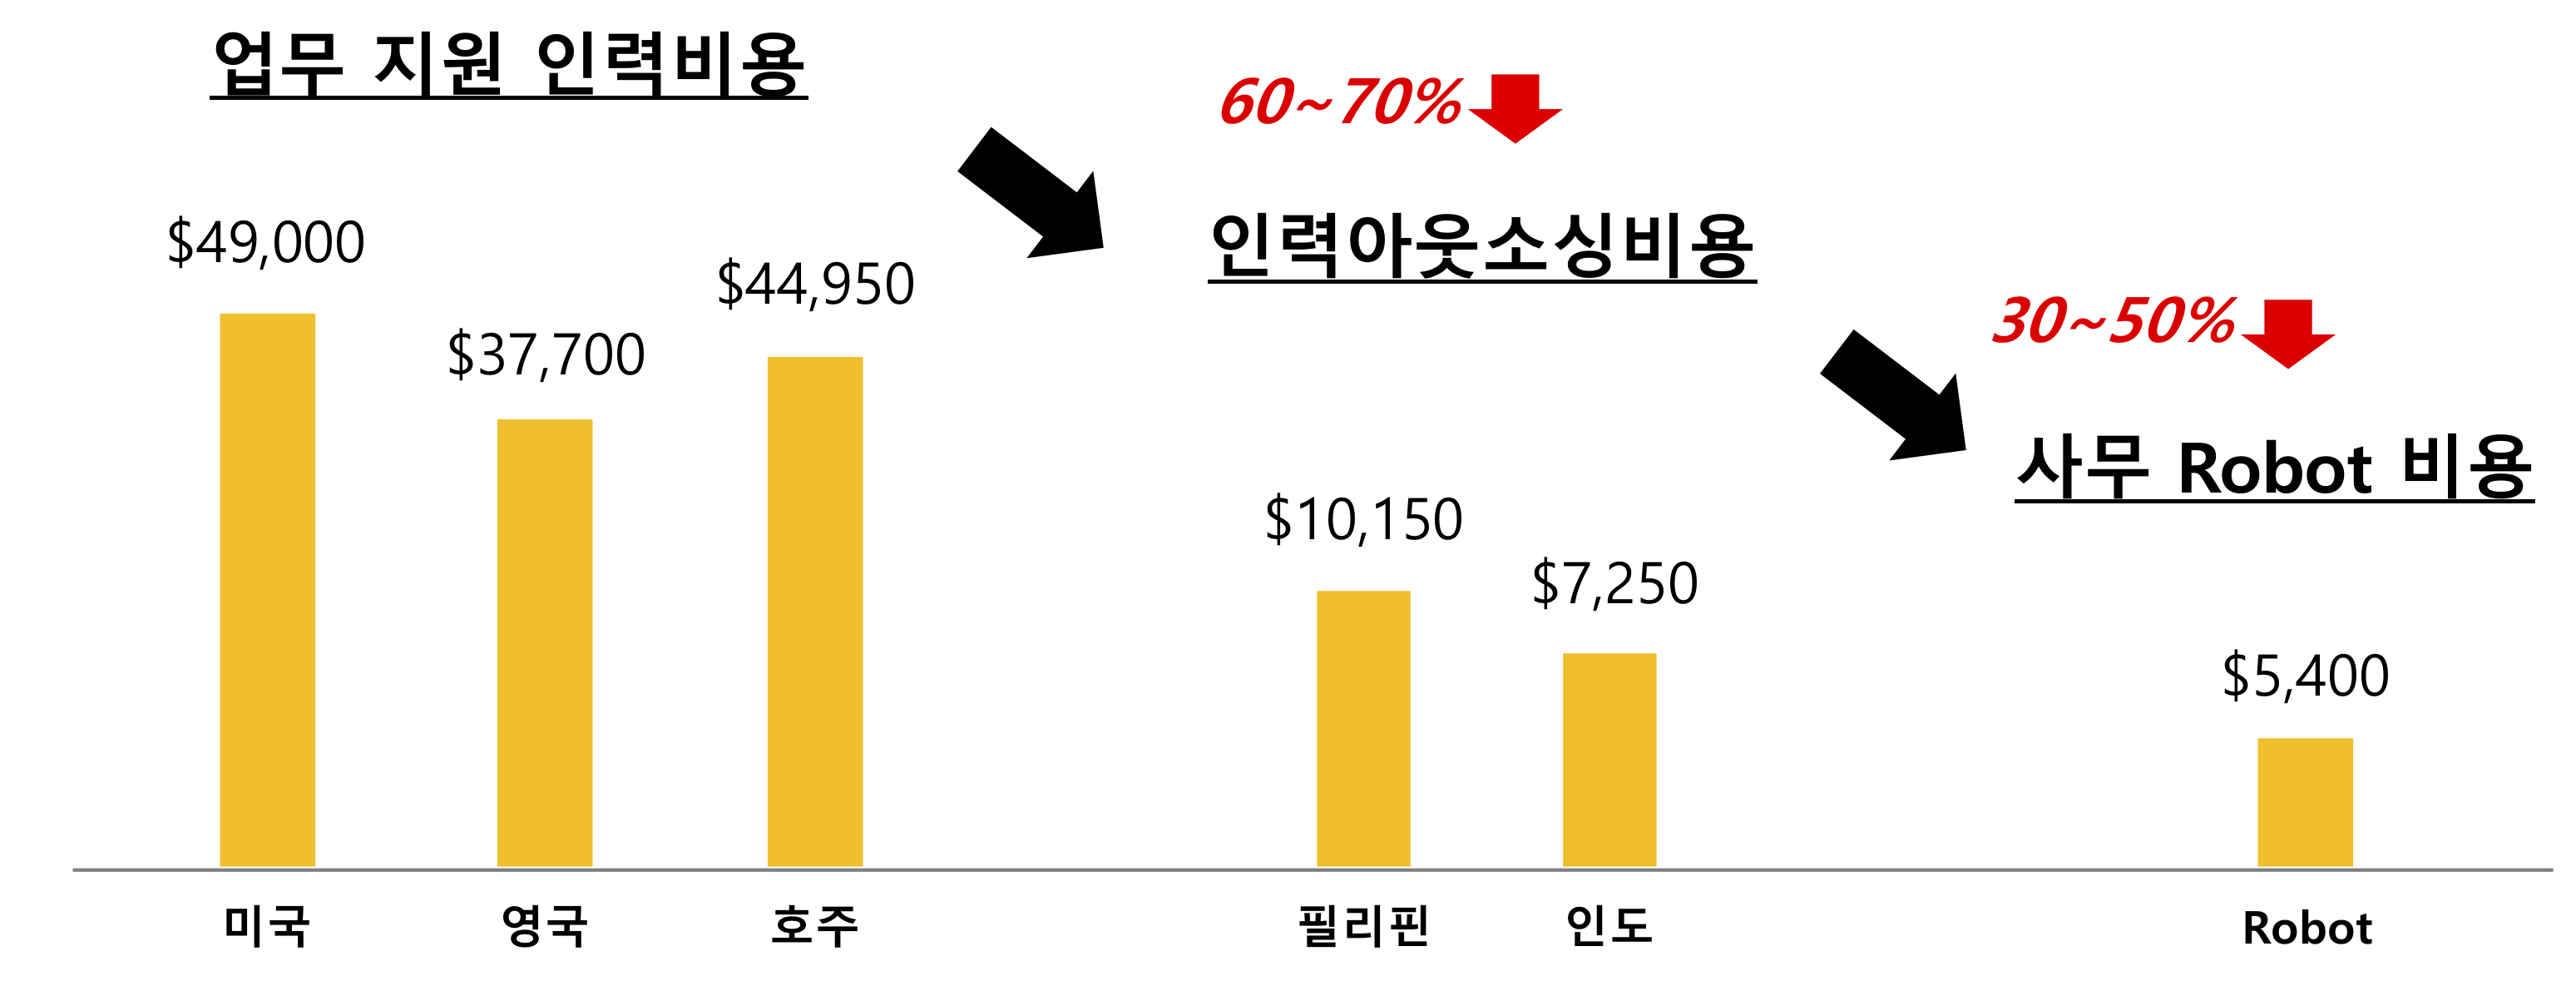
\includegraphics[width=1\linewidth]{fig/the-end-of-outsourcing} \end{center}

그러나 현재 Apple 회사에서 개발한 Siri, Amazon의 Alexa, Google의 Google
Assistant 등 인공지능을 활용한 개인 비서의 출범으로 시작하여 많은
기업들은 채팅로봇 (챗봇)을 개발하여 근무시간 외에도 고객들이 문의를 할
수 있게 고객센터의 효율성을 높였다. 회사에서 제공하는 서비스가 많으면
그에 부합한 조건도 많아질 것이며 한 직원이 고객들에게 정확히 어느
서비스를 제공해야 하는지 놓칠 수도 있다. 그러나 데이터와 인공지능 기술을
사용해 분석하면 유의미한 관계를 추출하고 이를 고객들의 요구 사항에 맞춰
그들이 충족하는 서비스를 제공할 수 있게 된다.

\hypertarget{industrial-robot}{%
\subsection{산업용 로봇}\label{industrial-robot}}

\begin{center}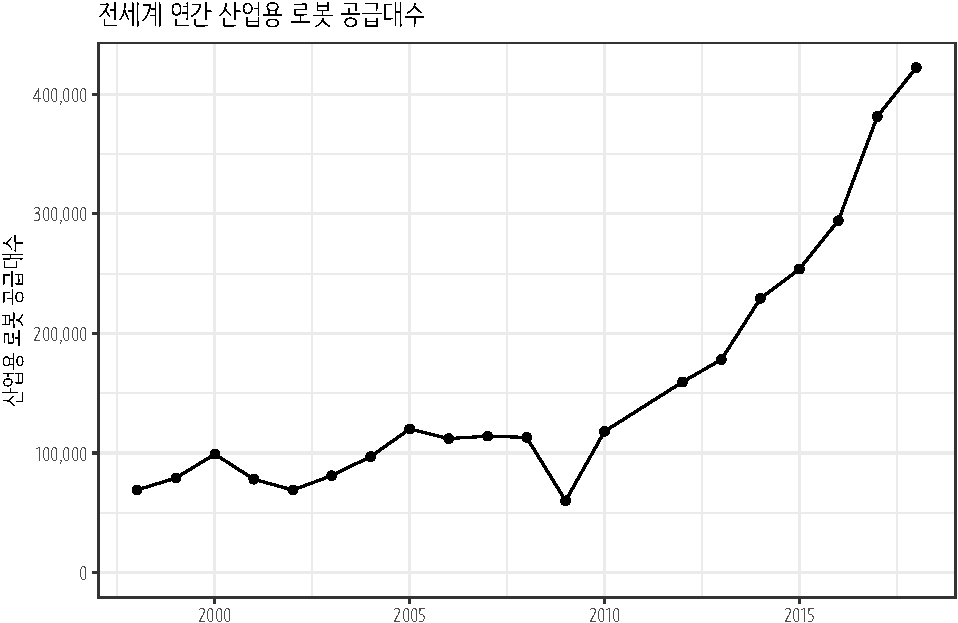
\includegraphics[width=1\linewidth]{paper_files/figure-latex/industrial-robot-1} \end{center}

산업용 로봇에 대한 기사\cite{ahlstrom_2019}에 따르면 2010년을 기점으로
8년 동안 산업용 로봇은 대략 300,000대 이상 공급되며 엄청난 성장세로
증가했다. 특히 2008년 금융위기 후 산업용 로봇 공급이 급격히 늘어난
추세를 확인할 수 있다. 산업용 로봇은 무거운 제품 또는 무한적으로
반복되는 과정을 사람들보다 효율적으로 처리할 수 있어 전에는 사람들이
많이 필요했던 작업들을 대신하기 시작했다.

\hypertarget{automation-result}{%
\section{일자리 변동 결과}\label{automation-result}}

생산성과 임금격차, 보울리의 법칙, 노동인력 참여율을 통해 확인되는 공통된
사항은 1980년 이후 일자리에 구조적인 변동이 생겼다는 점이다. 데이터
과학을 활용하여 생산성과 임금격차 데이터, 노동소득 분배율 데이터,
노동인력 참여율 데이터를 받아 시각화하게 되면 이러한 변화를 직관적으로
확인할 수 있다.

\hypertarget{wage-productivity-gap}{%
\subsection{생산성과 임금 격차}\label{wage-productivity-gap}}

\begin{center}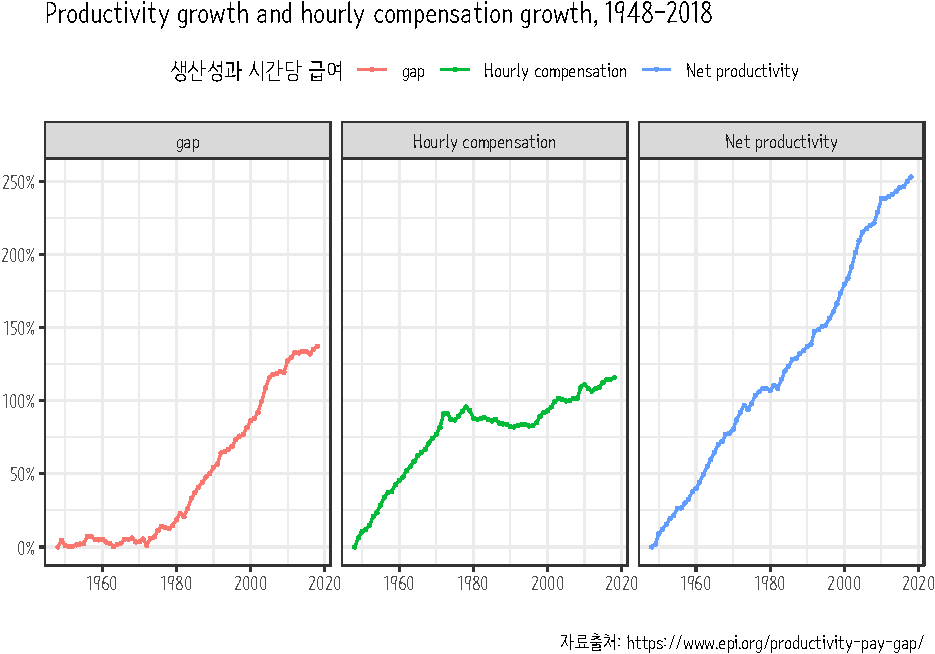
\includegraphics[width=1\linewidth]{paper_files/figure-latex/productivity-gap-1} \end{center}

그동안 생산성이 오르면 임금도 따라 오른다고 믿어왔다. 그러나 경제 정책
연구소 (Economic Policy
Institute)\cite{economic_policy_institute_2019}는 생산성이 오른다고
임금도 같이 따라 오르지는 않는다는 현상이 1979년부터 심화되고 있다는
최근 연구 결과를 발표했다. 데이터\cite{bivens2014raising}를 통해
분석해본 결과 시간당 임금은 1980년부터 별다른 변동이 없으나 순 생산성은
1980년 이전과 마찬가지로 꾸준히 오르고 있다. 따라서, 시간당 임금과
생산성의 차이는 지속적으로 벌어지고 있는 현실을 볼 수 있다.

\hypertarget{bowley-law}{%
\subsection{보울리 법칙(Bowley's Law)}\label{bowley-law}}

임금과 노동생산성 간 격차의 지속적 증가는 노동소득분배율 (labour income
share)의 감소로 연결된다. 노동소득분배율은 총국민소득 중 노동소득이
차지하는 비중이며 보울리의 법칙은 경제성장이나 발전과는 상관없이
노동소득분배율은 장기적으로 일정하다는 가설\cite{lee_2014}이다. 그러나
최근에 이 가설에는 변화가 생기기 시작했다.

\begin{center}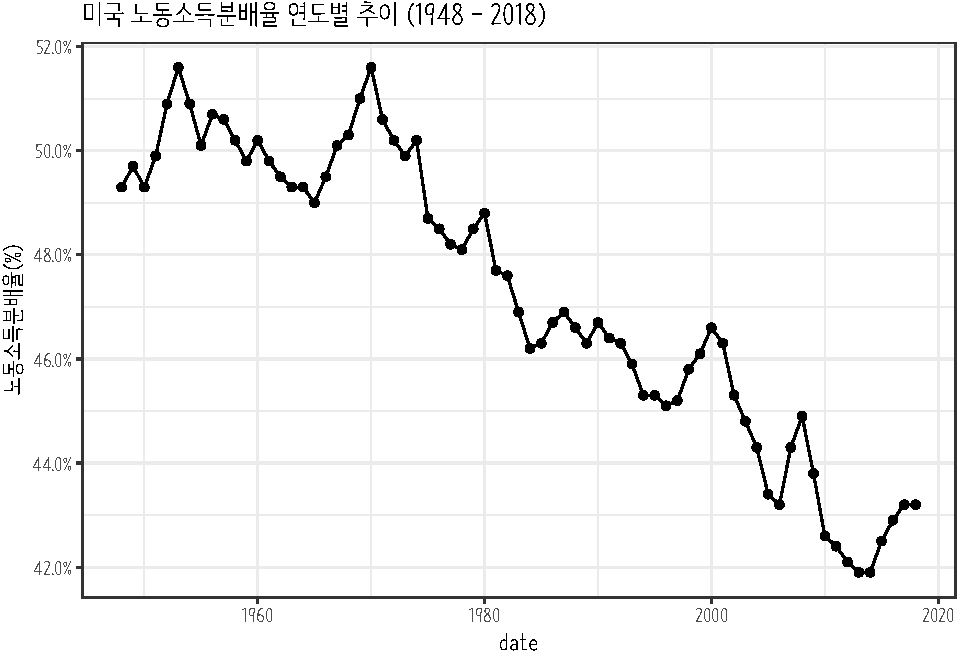
\includegraphics[width=1\linewidth]{paper_files/figure-latex/labor-share-us-1} \end{center}

FRED Economic Data \footnote{\href{https://fred.stlouisfed.org/series/W270RE1A156NBEA}{Shares
  of gross domestic income: Compensation of employees, paid: Wage and
  salary accruals: Disbursements: to persons (W270RE1A156NBEA)}}
데이터를 분석해본 결과 미국은 1970년부터 2010 년까지 노동소득분배율이
50\%에서 42\% 이하로 가파른 속도로 감소했다. International Labor
Organization (ILO)의 세계 임금 보고서\cite{ilo2015labour}에는 산업구조
변화와 기술 변화, 세계화, 금융화(financialization), 노동시장과
복지정책의 약화 등이 감소 원인이라고 제시하고 있다.

\hypertarget{labor-participation}{%
\subsection{노동인력 참여율}\label{labor-participation}}

\begin{figure}

{\centering \includegraphics[width=1\linewidth]{paper_files/figure-latex/labor-share-test-1} 

}

\caption{TESTING}\label{fig:labor-share-test}
\end{figure}

\href{https://research.stlouisfed.org/docs/api/api_key.html}{Federal
Reserve Bank of ST. Louis}에서 제공하는 데이터를 받아 분석한 결과
1965년부터 가파른 속도로 노동참여율이 증가했으나 2000년은 정점으로
하락하 기 시작했다. 산업용 로봇은 2010년부터 가파른 속도로 공급 되었으나
노동참여율은 2010년 이후 가파른 속도로 감소했다. 산업용 로봇과 노동
참여율의 관계는 반비례 적이며 인공지능의 발전으로 두 부문의 차이는 커질
전망이다.

\hypertarget{human-and-ai-reality}{%
\section{사람과 인공지능의 현실}\label{human-and-ai-reality}}

\hypertarget{human-and-ai-compare}{%
\subsection{사람과 인공지능 비교}\label{human-and-ai-compare}}

\begin{table}[H]
\centering
\resizebox{\linewidth}{!}{
\begin{tabular}{lll}
\toprule
속성 & 사람 & 기계\\
\midrule
\rowcolor{gray!6}  속도 & 상대적으로 느림 & 탁월함\\
경격출력 & 상대적으로 약함 & 일관된 작업에 우수성을 보임\\
\rowcolor{gray!6}  일관성 & 믿을 수 없는 학습능력과 피로 & 일관되고 반복적인 작업에 이상적임\\
정보처리능력 & 주로 한개 채널 & 멀티 채널\\
\rowcolor{gray!6}  기억 & 원칙과 전략에 좋음. 다재다능하고 혁신적임 & 문자 그대로 재현하는데 이상적임, 형식적임\\
\addlinespace
추론 계산 & 귀납적, 프로그램하기 더 좋고, 느리고, 오류 수정 좋음 & 연역적, 프로그램하기 귀찮고, 빠르고 정확, 오류 수정 나쁨\\
\rowcolor{gray!6}  감지(sensing) & 넓은 감지 반경, 다기능, 분별력 & 정량적 평가에 좋지만, 패턴인식에는 나쁨\\
인지(perceiving) & 변화에 더 잘 대응 & 잡음에 취약하여 변화에 잘 대응 못함.\\
\bottomrule
\end{tabular}}
\end{table}

사람과 기계는 서로 잘하는 영역이 나눠져 있었다. 단어를 찾거나 글자 수를
세는 단순하고 반복적인 작업은 컴퓨터에게는 쉬운 작업이다. 반면, 논문이나
책을 읽는 것은 현재 기술로는 한계가 있다. 인간은 지루하고 반복된 문제를
해결하는 데 적합하지 않지만 컴퓨터는 추상적이고 일반화하는 작업에
적합하지 않다. 이 사실은 1970년대 미국 카네기 멜론 대학 (CMU) 로봇
공학자 한스 모라벡(Hans Moravec) 교수의 모라벡의 역설(Moravec's
paradox)로 잘 알려져 있다.

\hypertarget{uxbaa8uxb77cuxbca1uxc758-uxc5eduxc124moravecs-paradox}{%
\subsection{모라벡의 역설(Moravec's
paradox)}\label{uxbaa8uxb77cuxbca1uxc758-uxc5eduxc124moravecs-paradox}}

한스 모라벡은 1970년대에 컴퓨터와 인간의 능력 차이를 역설적으로 표현하며
다소 직설적인 발언을 했다 \footnote{`It is comparatively easy to make
  computers exhibit adult level performance on intelligence tests or
  playing checkers, and difficult or impossible to give them the skills
  of a one-year-old when it comes to perception and mobility.'}. 즉,
인간은 걷기, 느끼기, 듣기, 보기, 말하기 등의 일상적인 행위는 매우 쉽게
할 수 있는 반면 복잡한 수식 계산 등을 하기 위해서는 많은 시간과 에너지를
소비해야 한다. 반대로 컴퓨터는 인간이 하는 일상적인 행위를 수행하기 매우
어렵지만 수학적 계산, 논리 분석 등은 쉽게 해결할 수 있다.

모라벡 역설의 사례로 최근 인공지능 학습의 난제중 하나를 꼽으라면 여전히
다음과 같은 분류 문제를 들 수 있다. 머핀과 치와와 혹은 아이스크림과
고양이를 분류 시켜야 하면 사람들은 쉽게 구분할 수 있으나 기계는 다양한
알고리즘을 사용하여 학습을 시켜 결과를 얻는다. 그러나 정확성은 높게
나오지 않는 경우가 많다.

\begin{center}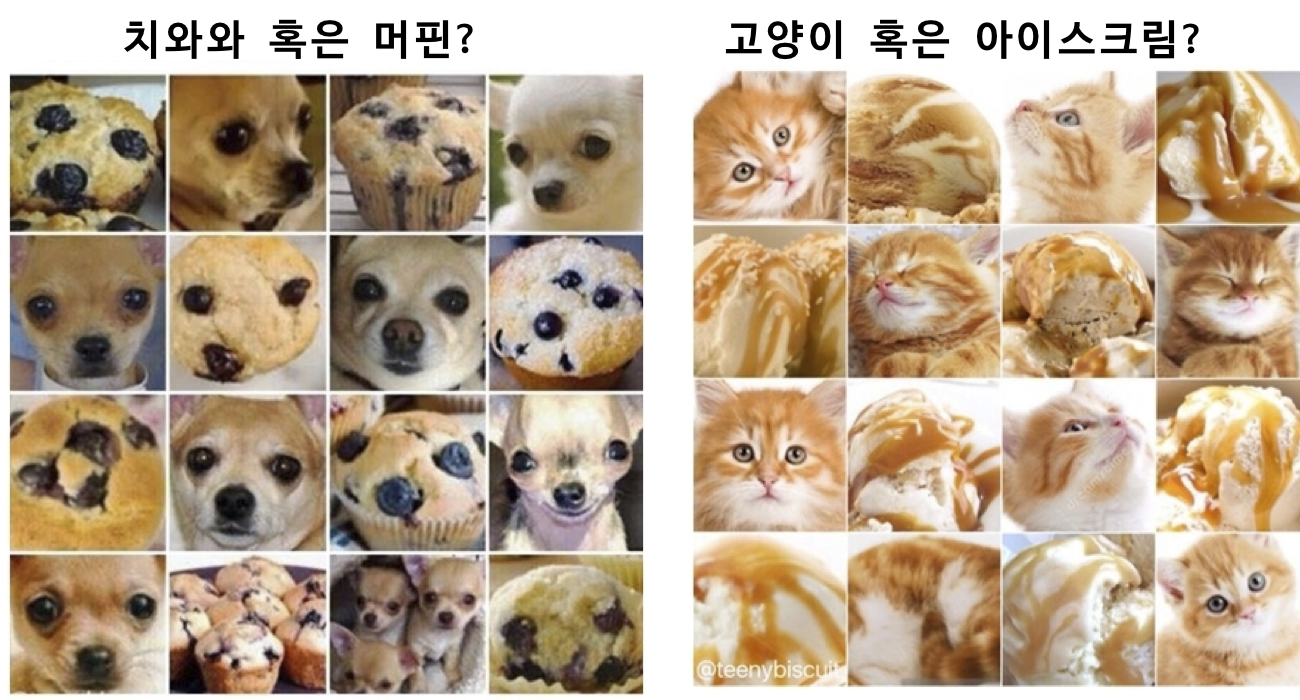
\includegraphics[width=1\linewidth]{fig/moravec-paradox} \end{center}

\hypertarget{chinese-room}{%
\subsection{중국어 방 주장}\label{chinese-room}}

중국어 방 혹은 중국인 방(영어: Chinese room) \cite{wikipedia_2019}은 존
설(John Searle) 이 튜링 테스트로 기계의 인공지능 여부를 판정할 수 없다는
것을 논증하기 위해 고안한 사고실험이다.

\begin{quote}
우선 방 안에 영어만 할 줄 아는 사람이 들어간다. 그 방에 필담을 할 수
있는 도구와 미리 만들어 놓은 중국어 질문과 질문에 대한 대답 목록을
준비해 둔다. 이 방 안으로 중국인 심사관이 중국어로 질문을 써서 넣으면 방
안의 사람은 준비된 대응표에 따라 답변을 중국어로 써서 심사관에게 준다.
\end{quote}

안에 어떤 사람이 있는지 모르는 심사관은 당연히 중국어를 할 줄 아는
사람이 있을 거라고 생각할 것이다. 그러나 안에 있는 사람은 중국어 질문을
이해하지 않고 주어진 표에 따라 대답할 뿐이다. 이를 통해 중국어로 질문과
답변을 받은 결과가 완벽해도 안에 있는 사람이 중국어를 정확히 이해했는지
판정하기 어렵다는 결 론을 얻는다. 이와 마찬가지로 지능이 있어서 질문
답변을 수행할 수 있는 기계가 있어도 그것이 지능을 가졌는지는
\textbf{튜링 테스트}로만 판정할 수 없다는 주장이다.

\begin{table}[H]
\centering
\resizebox{\linewidth}{!}{
\begin{tabular}{lll}
\toprule
인공지능 & 컴퓨터 & 인간\\
\midrule
\rowcolor{gray!6}  중국어 방 & 하드웨어 & 인간의 외형적인 몸체\\
영어만 할 줄 아는 사람 & 소프트웨어 & 인간의 지능\\
\rowcolor{gray!6}  중국어로 된 질문 & 입력(Input) & 인간이 외부에서 접할 수 있는 자극\\
중국어로 된 답변 & 출력(Output) & 인간이 외부에서 접한 자극에 대한 반응\\
\rowcolor{gray!6}  질문\&대답 목록 & 데이터베이스(Database) & 습득된 기억\\
\bottomrule
\end{tabular}}
\end{table}

결국 다음과 같이 컴퓨터, 인간, 인공지능을 비교할 수 있다. 중국어 방을
인간으로 비유하면 외형적인 몸체이고 컴퓨터를 하드웨어라고 가정하면
질문과 답변을 입출력으로 정의할 수 있으며 질문\&대답 목록과 처리 규칙을
담은 알고리즘을 데이터베이스/알고리즘, 습득된 경험, 지식, 지능으로
대응할 수 있다.

\hypertarget{man-human-boundary}{%
\section{사람과 기계 업무 분장}\label{man-human-boundary}}

모라벡의 역설 또는 중국어 방 예시처럼 인공지능은 시행 착오를 통해 학습을
한다. 그 결과, 새로운 환경에 마주치면 예상 밖의 결과를 반환 할 가능성이
있다. 실제로 달에 사람을 보내는 아폴로 계획에서 사람과 기계의 역할을
어떻게 구분하는 것이 좋은지는 오랜 동안 사람과 기계의 업무 분장에 대해
논란이 되었던 대표적인 사례이다. 그러므로 모든 결정을 인공지능에
의존하는 대신 사람과 협동해 업무를 분리해서 처리하는 것이 효율적이다.

예를 들면(Korea Telecom)에서 출시한 `스마트 팩토리'는 인공지능,
사물인터넷 (IOT, Internet of Things) 등 네트워크 기술을 사용해 생산
업무를 자동화 하는 공장이다 \textbf{{[}출처: 4차 산업혁명과 직업의
미래{]}}. 최근에 5세대 이동 통신 (5G)의 출범으로 통신 속도가 급격히
빨라져 인공지능 기술 기계에 신속히 적용할 수 있게 되었다. 그 결과 산업용
로봇을 사용하여 데이터를 수집하고 분석하고 인공지능 기술을 사용해 스스로
학습해서 실무에 적용 시키기 시작했다. 만약 설비의 과부하로 고장 또는
이상이 생기기 전에 이를 인식하고 생산을 중단하거나 컨트롤 타워에 신호를
보내 위기를 모면하는 등 같이 일하는 작업자 옆에서 보조 업무를 수행하며
위험성을 감지해 안정을 지켜준다. 여기서 주목해야할 점은 컨트롤 타워이다.
생산라인에 문제가 생기는 사유는 다양하며 모두가 안정을 위협하지는
않는다. 그러나 인공지능을 사용한 로봇은 `문제'라는 이유로 모든 생산을
중단하면 큰 손해를 본다. 그래서 문제를 인식하면 기계가 직접 결정하는
대신 업무에 능숙한 사람에게 질문을 주고 그들이 판단한 후 기계가 적용할
수 있게 업무를 분산시켜 문제를 해결 하면 효율적이고 생산적이다.

그 외에도 미국 전기 자동차 회사 테슬라 (Tesla) 또는 IT 기업 구글
(Google)은 인공지능을 활용해 무인 자동차 개발을 꾸준히 해오고 있다.
테슬라는 이미 2014년 9월에 반자동 운전 보조 장치가 탑재되어 있는
서비스를 출시해 상용화하기 시작했다. 여기서도 주목해야할 부분은
`반자동'이다. 자율주행 분야의 인공지능 기술은 오랜 시간 동안 현재
존재하는 많은 데이터를 학습시킨다. 그럼에도 불구하고 데이터에 존재하지
않던 문제가 생기면, 예를 들면 갑자기 다른 차선에서 예상치 못한 일들이
벌어진다면, 인공지능은 새로 접하는 데이터를 인식을 못해 파격적인 결과를
불러올 수 있다. 반대로 운전을 하다 사람의 실수로도 치명적인 결과를
불러올 수 있다. 그러므로 인공지능에 모두 의존하기 보다는 사람이 꾸준히
관찰하며 인공지능 기술을 사용해야 한다.

\begin{center}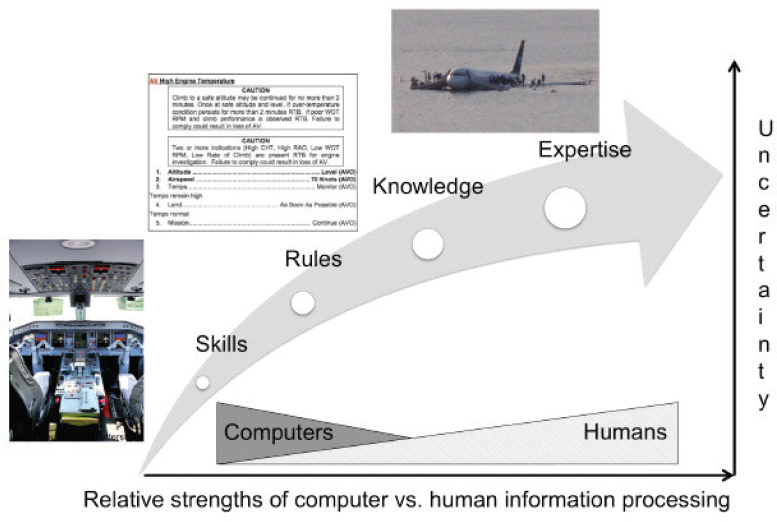
\includegraphics[width=0.77\linewidth]{fig/role-allocation-skill-rules-experties} \end{center}

\begin{verbatim}
test-rmarkdown}
srke_tbl <- "| 인지 작업 (cognitive behavior/task) | 자동화 정도(degree of automation) |
|:--------------------------:|--------------------------|
| 기량(skill-based)        | 자동화에 최적화됨. 물론 내외부 상태와 오류 피드백에 대한 신뢰성있는 센서를 가정 |
| 규칙(rule-based)         | 자동화 가능한 대상. 물론 규칙집합이 잘 만들어지고 테스트된 것을 가정 |
| 지식(knowledge-based)    | 일부 자동화를 통해 데이터를 조직화하고, 필터링하고, 합성하는데 도움을 줌 |
| 전문적 식견(expertise)   | 사람이 가장 잘 할 수 있지만, 팀동료로 자동화 기계를 통해 도움을 받을 수 있음 |"

read_markdown(srke_tbl) %>% 
  knitr::kable(format = "latex", booktabs = TRUE) %>% 
  kable_styling(latex_options = c("striped", "scale_down"))
\end{verbatim}

듀크 대학과 MIT 소속 매리 커밍스(Mary Cummings) 교수는 기존 (S-R-K,
Skill- Rule-Knowledge) 틀에 E(Expertise)를 추가하여 기계는 스킬(Skill)과
규칙(Rule)에서는 뛰어나지만 지식(Knowledge)과 전문성(Expertise)에서는
사람이 기계보다 우월하다는 주장을 했다. 커밍스 교수는 이를 `사람 감독
아래 제어'(Human Supervisory Control) 로 명명하였다.

\begin{center}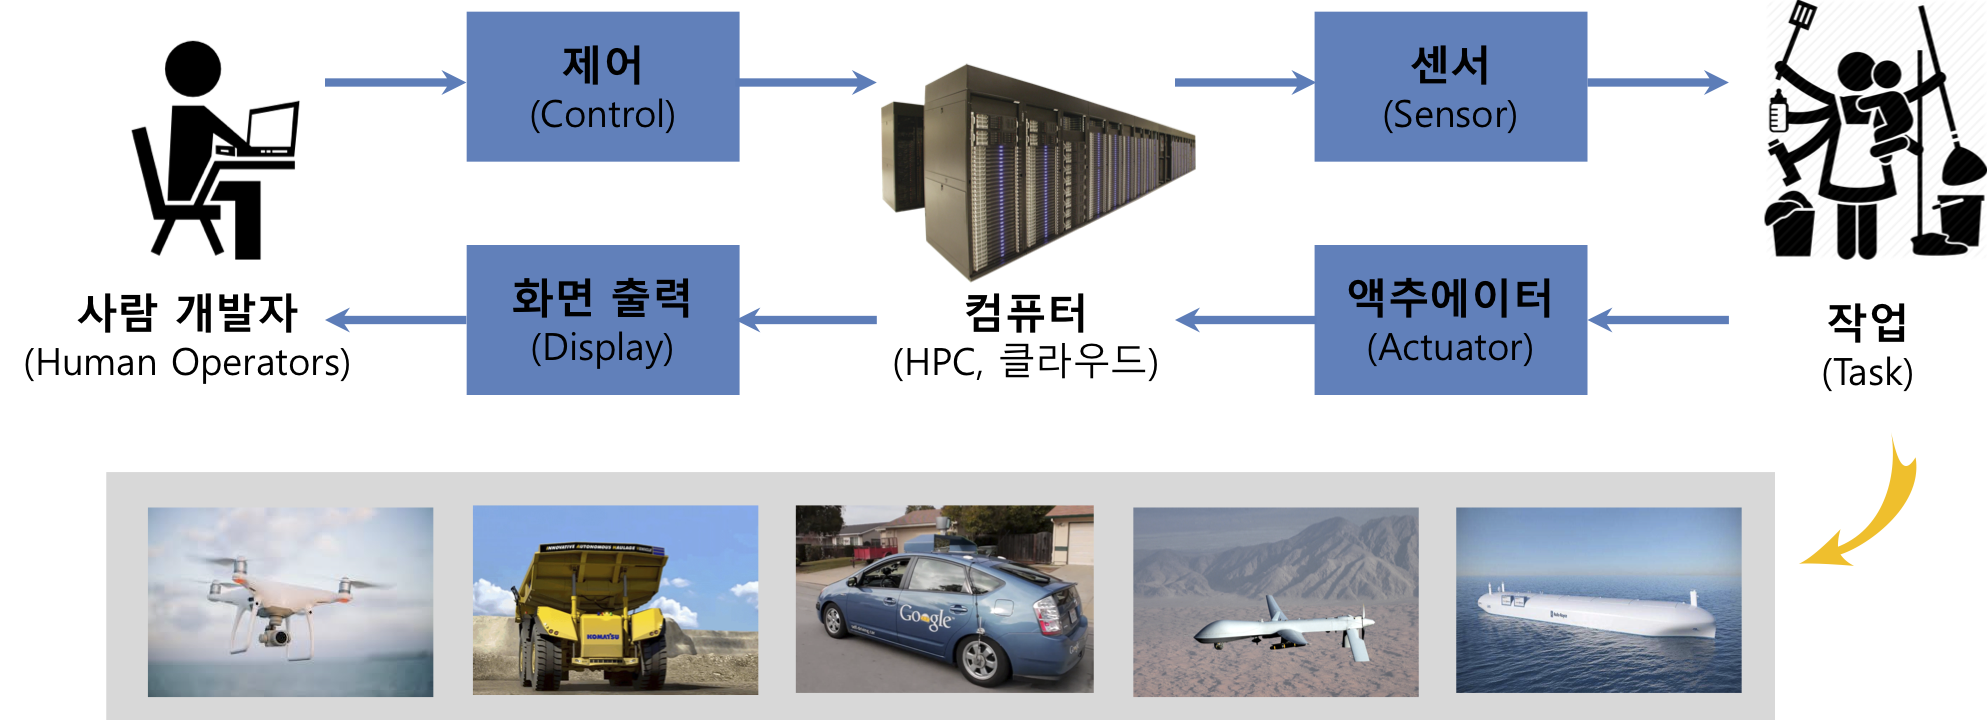
\includegraphics[width=0.77\linewidth]{fig/human-supervisory-control} \end{center}

최근 인공지능 기술을 탑재한 기계는 드론, 무인 자동차, 무인 화물자동차,
무인 비행기, 무인 선박 모두 센서와 액추에이터를 통해서 자동으로 설정한
목표를 달성하게 되어 있지만 이는 중앙 컴퓨터의 제어를 받는다. 중앙
컴퓨터 제어는 결국 사람이 화면을 보고 제어 로직을 심어둔 것이며 인공지능
혼자 모든 것을 해결하기는 아직 이르다는 주장이다.

\hypertarget{conclusion}{%
\section{결어}\label{conclusion}}

기술 발전으로 컴퓨터 처리 속도가 빨라지면서 인공지능 상용화에 가속도가
붙기 시작했다. 전에는 수많은 사람들이 작업해서 나왔던 결과를 이제는 미리
학습한 인공지능을 사용해 최소의 인원으로 문제를 빨리 해결할 수 있게
되었다. 그리고 기계는 같은 작업을 계속 반복해도 지치지 않고 꾸준히
생산성을 유지한다. 그 결과, 생산업체, 콜센터 등 많은 인원이 필요하고
반복적으로 비슷한 업무를 하는 작업을 인공지능을 통해 저렴하고 효율적으로
업무를 대체하려고 했다. 그러나, 인공지능을 분별없이 사용하면 혼란을 겪게
될 것이다. 커밍스 교수가 말했듯이 기계는 전문성이 사람에 비해 낮으므로
기계에만 의존하고 모든 결정을 내리면 기업 또는 사용자들은 손해를 볼
것이다. 인공지능은 오랜 학습을 거쳐 만들어진 기술이다. 그러므로 학습을
하면서 인식을 못했던 문제들을 현장에서 발견했을 때 이것이 긍정적인
문제인지 아니면 부정적인 문제인지 결정을 못하면 기업인 경우 적자를 볼
수도 있는 경우가 생길 수도 있다. 그래서 인공지능에 모든 것을 의존하기
보다는 전문성을 가지고 있는 사람들의 제어 아래 사용하는 것이 더
효율적이다. 마지막으로, 인공지능을 모든 업무를 대신하려고 만드는
것보다는 사람들을 보조하는 역할로 기술을 활용해 효율적인 판단을 할 수
있는 방향으로 개발해야 한다. 이제는 기계를 통한 자동화의 본질을 직시하고
기계와 인간이 공존하며 만들어가는 새로운 패러다임을 받아들일 준비를 할
시점이 되었다.

\bibliographystyle{spbasic}
\bibliography{bibliography.bib}

\end{document}
